\section{結果}
\subsection{近接2粒子ホログラムの検証実験}
この実験で記録したホログラムと,そのフーリエ変換で得たスペクトル分布の例を Fig. \ref{fig:stripePatternExpExample} に示す.あ

\begin{figure}[htbp!]
    \centering
    \begin{subfigure}[c]{0.45\linewidth}
        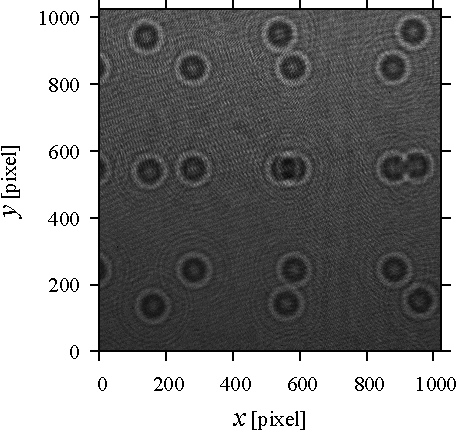
\includegraphics[width=\linewidth]{./Figure/4_Results/stripe_pattern_experiment/recorded_data/a.pdf}
        \caption{Recorded hologram image}
        \label{fig:stripePatternExpExample:a}
    \end{subfigure}
    \hfill
    \begin{subfigure}[c]{0.45\linewidth}
        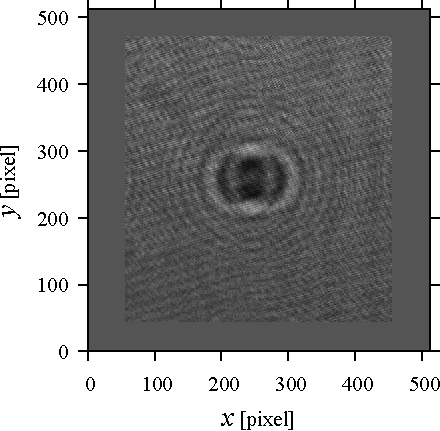
\includegraphics[width=\linewidth]{./Figure/4_Results/stripe_pattern_experiment/recorded_data/b.pdf}
        \caption{Cropped hologram image of Fig. \ref{fig:stripePatternExpExample:a}}
        \label{fig:stripePatternExpExample:b}
    \end{subfigure}

    \begin{subfigure}[b]{0.8\linewidth}
        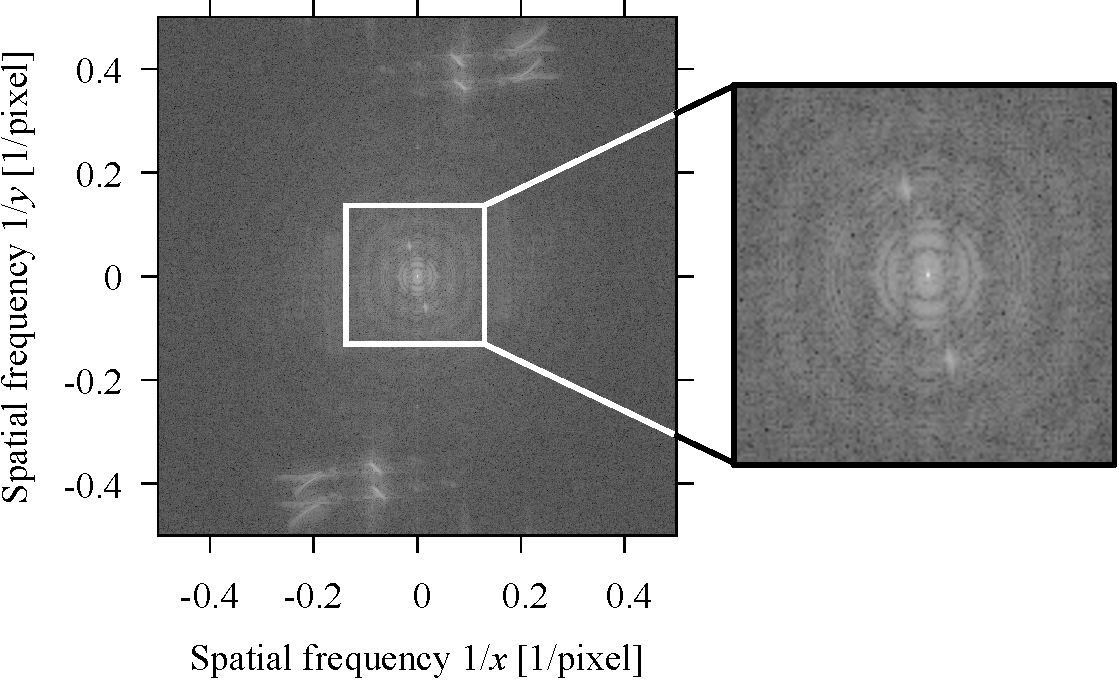
\includegraphics[width=\linewidth]{./Figure/4_Results/stripe_pattern_experiment/recorded_data/c.pdf}
        \caption{Computationally calculated spectrum of the hologram Fig. \ref{fig:stripePatternExpExample:b}}
        \label{fig:stripePatternExpExample:c}
    \end{subfigure}

    \caption{Example of a hologram and its spectrum. } 
    \label{fig:stripePatternExpExample}
\end{figure}

\begin{figure}[htbp!]
    \centering
    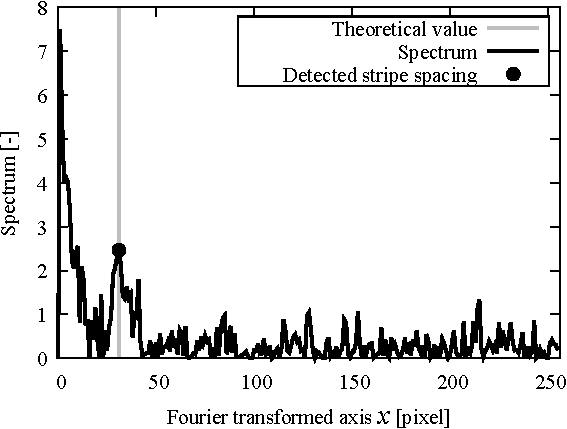
\includegraphics[width=0.8\linewidth]{./Figure/4_Results/stripe_pattern_experiment/stripe_pattern_exp_exam_peak.pdf}
    \caption{}
    \label{fig:stripePatternExperiment}
\end{figure}

\begin{figure}[htbp!]
    \centering
    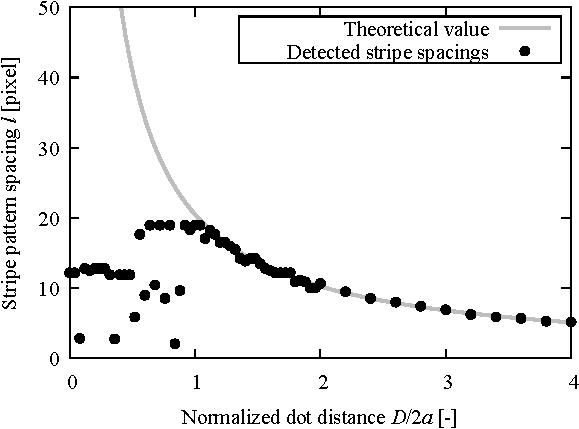
\includegraphics[width=0.8\linewidth]{./Figure/4_Results/stripe_pattern_experiment/stripe_pattern_exp_final_result.pdf}
    \caption{}
    \label{fig:stripePatternExperiment}
\end{figure}



\subsection{水滴近接検出モデルの性能評価および実験データに対する推論}

\begin{figure}[H]
    \centering
    \begin{subfigure}[c]{0.45\linewidth}
        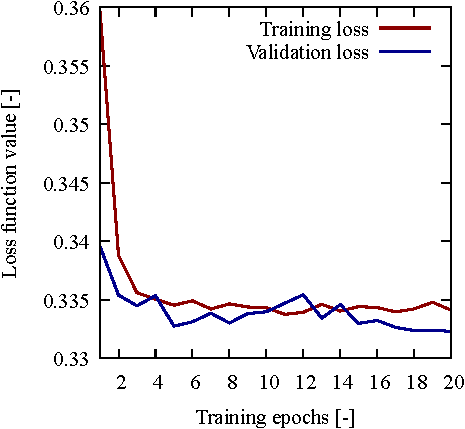
\includegraphics[width=\linewidth]{./Figure/4_Results/training/loss_fft.pdf}
        \caption{Loss improvement of the FFT-preprocessed model}
        \label{fig:stripePatternExpExample:a}
    \end{subfigure}
    \hfill
    \begin{subfigure}[c]{0.45\linewidth}
        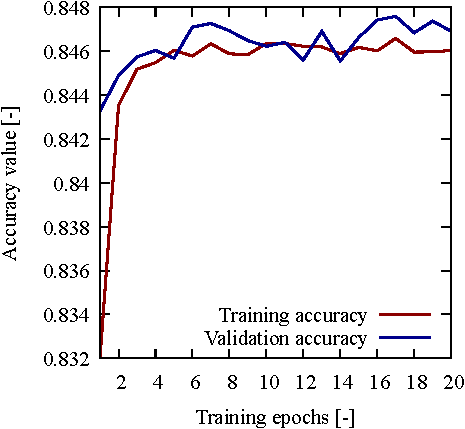
\includegraphics[width=\linewidth]{./Figure/4_Results/training/acc_fft.pdf}
        \caption{Accuracy improvement of the FFT-preprocessed model}
        \label{fig:stripePatternExpExample:b}
    \end{subfigure}

    \caption{Training results of the FFT-preprocessed model; the model was trained with the dataset of the FFT-preprocessed holograms. The stripe patterns of the proximity droplet holograms were enhanced by the FFT preprocessing, and they can be seen on the center of the spectrum.} 
    \label{fig:stripePatternExpExample}
\end{figure}

\begin{figure}[H]
    \centering
    \begin{subfigure}[c]{0.45\linewidth}
        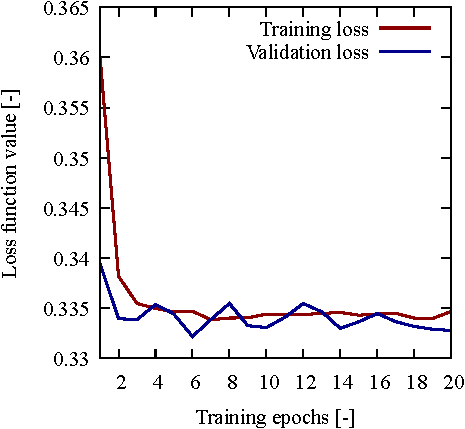
\includegraphics[width=\linewidth]{./Figure/4_Results/training/loss_raw.pdf}
        \caption{Loss improvement of the raw-input model}
        \label{fig:stripePatternExpExample:a}
    \end{subfigure}
    \hfill
    \begin{subfigure}[c]{0.45\linewidth}
        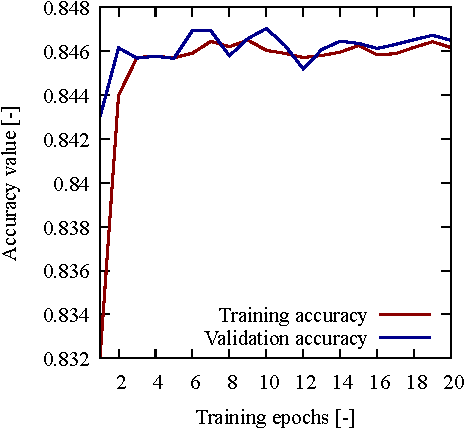
\includegraphics[width=\linewidth]{./Figure/4_Results/training/acc_raw.pdf}
        \caption{Accuracy improvement of the raw-input model}
        \label{fig:stripePatternExpExample:b}
    \end{subfigure}

    \caption{Training results of the raw-input model; the model was trained with the dataset of the raw holograms. The model can detect the proximity droplets without the FFT preprocessing because Fourier transform is a reversible operation.} 
    \label{fig:stripePatternExpExample}
\end{figure}

\begin{figure}[H]
    \centering
    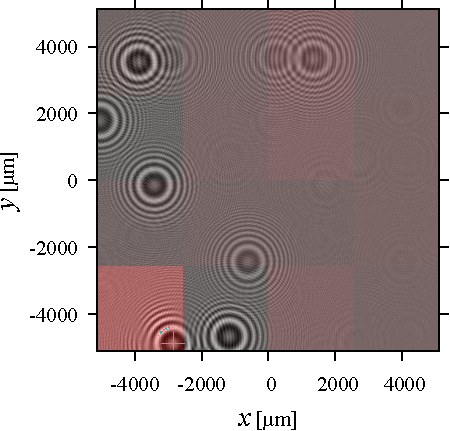
\includegraphics[width=0.8\linewidth]{./Figure/4_Results/training/outholo.pdf}
    \caption{Example of the inference result of the raw-input model. The proximity droplets are indicated by the green cross symbol. The shade of red overlay indicates the confidence of the model, and the confidence value on the green cross symbol partial area is \num{0.539}. This output image is contrast-enhanced for visualization.}
    \label{fig:stripePatternVector}
\end{figure}

\begin{figure}[H]
    \centering
    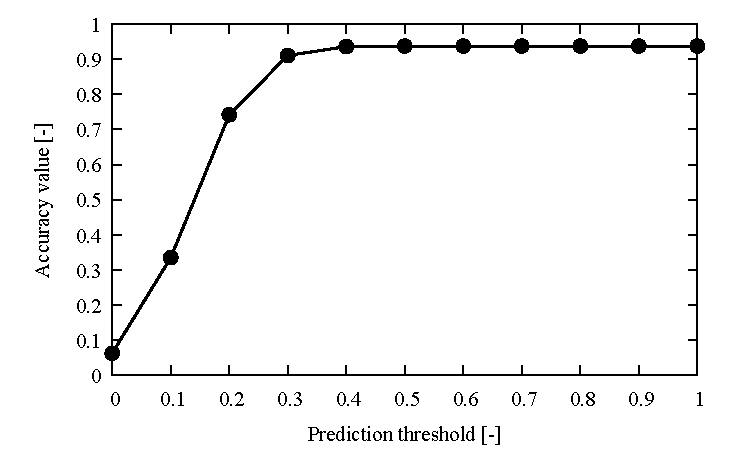
\includegraphics[width=0.8\linewidth]{./Figure/4_Results/training/acc_threshold.pdf}
    \caption{Accuracy value for each threshold value. The threshold value of \num{0.5} is the default value.}
    \label{fig:stripePatternVector}
\end{figure}

\begin{figure}[H]
    \centering
    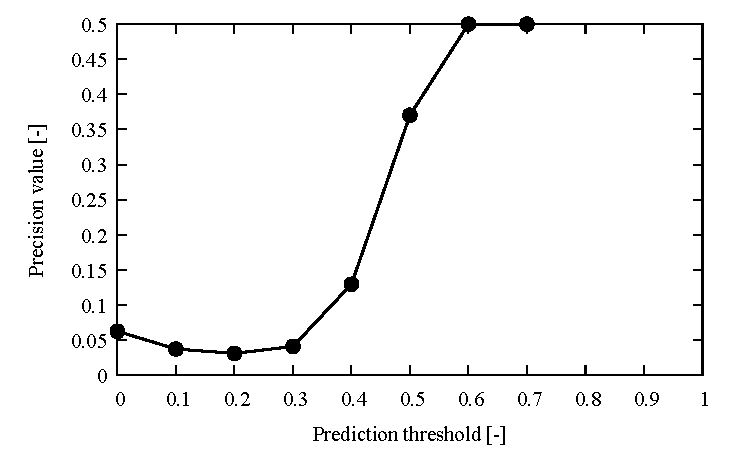
\includegraphics[width=0.8\linewidth]{./Figure/4_Results/training/precision_threshold.pdf}
    \caption{Precision value for each threshold value. The threshold value of \num{0.5} is the default value.}
    \label{fig:stripePatternVector}
\end{figure}

\begin{figure}[H]
    \centering
    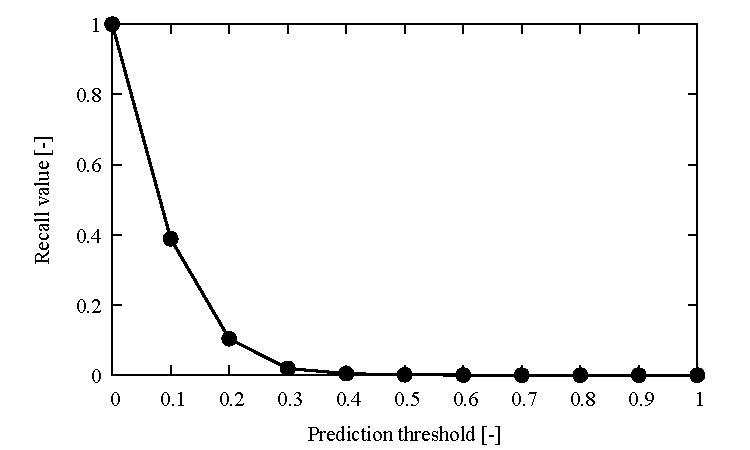
\includegraphics[width=0.8\linewidth]{./Figure/4_Results/training/recall_threshold.pdf}
    \caption{Recall value for each threshold value. The threshold value of \num{0.5} is the default value.}
    \label{fig:stripePatternVector}
\end{figure}

\begin{figure}[H]
    \centering
    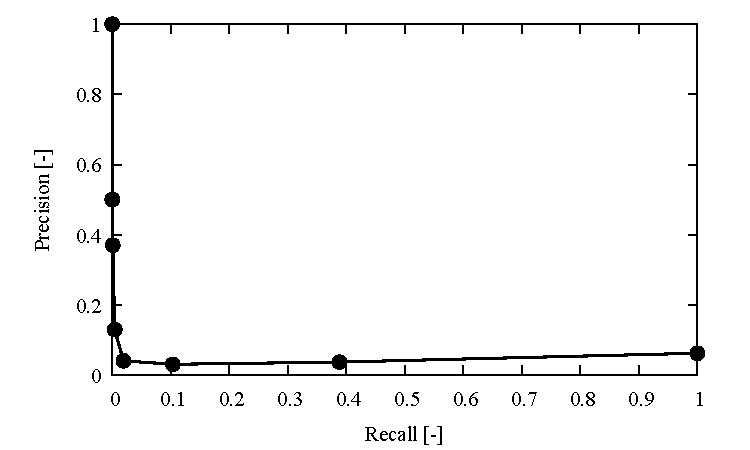
\includegraphics[width=0.8\linewidth]{./Figure/4_Results/training/prcurve.pdf}
    \caption{Precision-Recall curve of the raw-input model; each point represents the correspondence between the Recall and Precision values for a given discrimination threshold. Thresholds are taken from 0 to 1 in increments of 0.1.}
    \label{fig:stripePatternVector}
\end{figure}

\subsection{衝突水滴組の軌跡再生}

\begin{figure}[H]
    \centering
    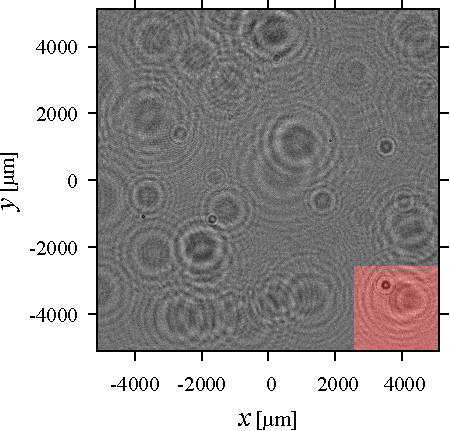
\includegraphics[width=0.8\linewidth]{./Figure/4_Results/exp/visout.pdf}
    \caption{Example of the inference result of the raw-input model, for the experimentally recorded hologram. The confidence value on the red shade area is \num{0.635}. This output image is contrast-enhanced for visualization.}
    \label{fig:expInfResult}
\end{figure}

\begin{figure}[H]
    \centering
    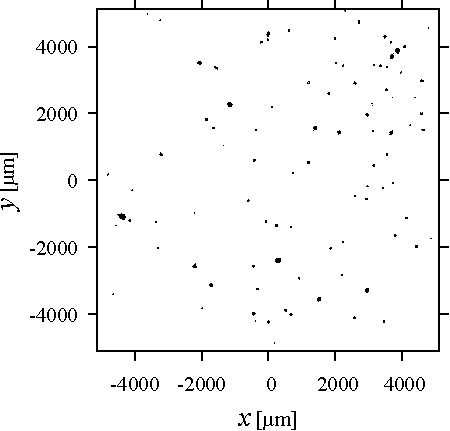
\includegraphics[width=0.8\linewidth]{./Figure/4_Results/exp/imp.pdf}
    \caption{$x$-$y$ projection of the reconstructed volume shown in Fig. \ref{fig:expInfResult}}
    \label{fig:expHoloImp}
\end{figure}

\begin{figure}[H]
    \centering
    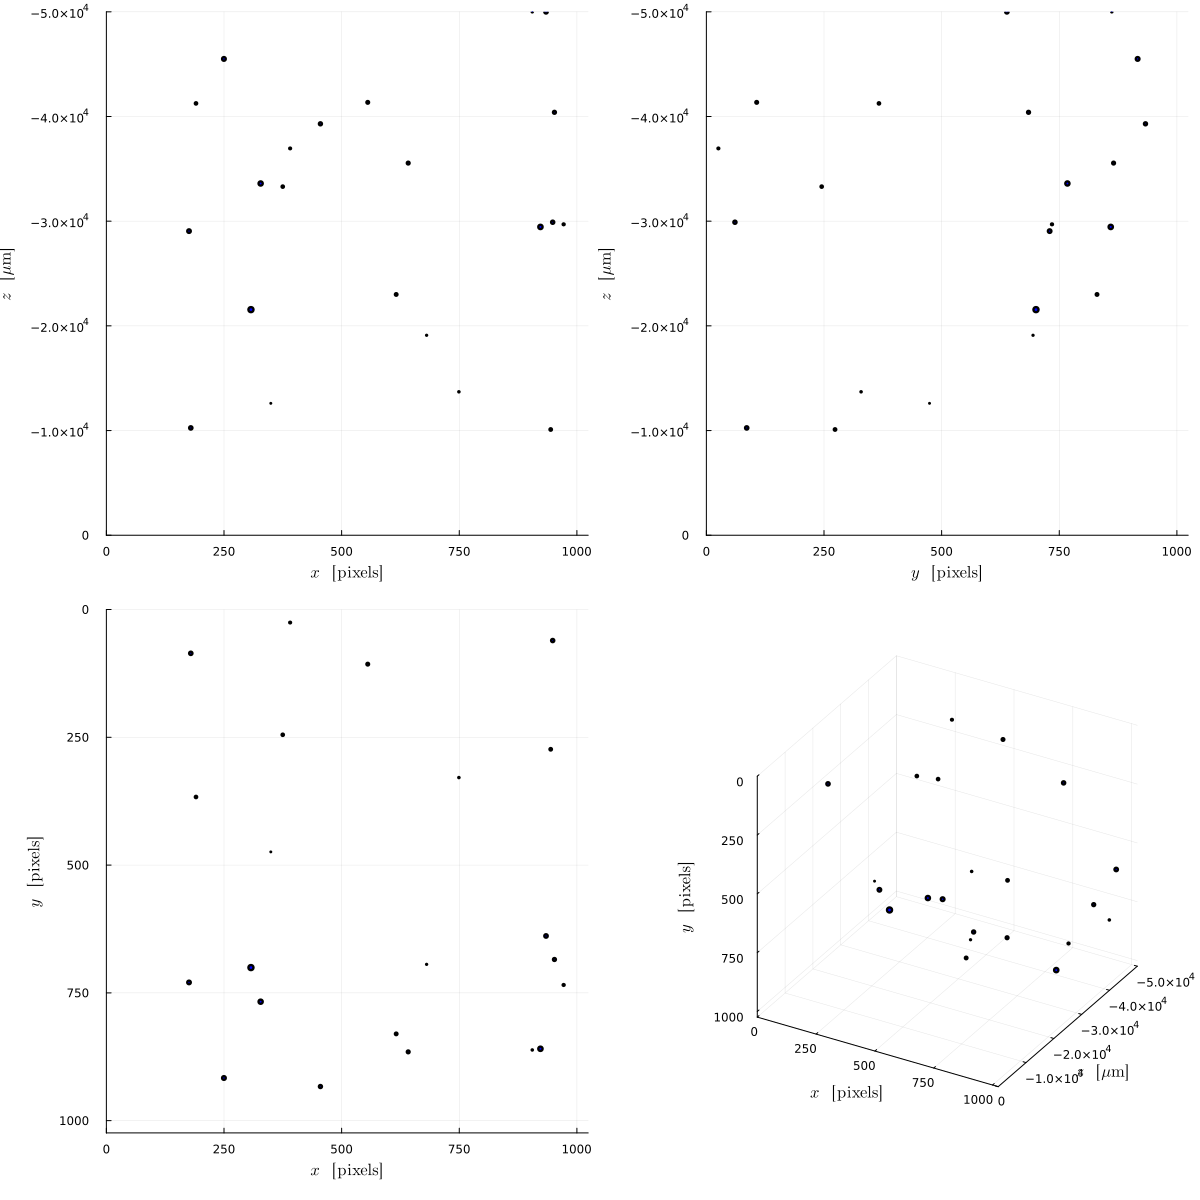
\includegraphics[width=0.8\linewidth]{./Figure/4_Results/exp/3dview.png}
    \caption{Three dimensional view of the reconstructed volume shown in Fig. \ref{fig:expInfResult}. There is an approaching droplet pair in the red shaded area shown in Fig. \ref{fig:expInfResult}.}
    \label{fig:3dview}
\end{figure}